% ------------------------------------------ %
%                      (2.1)                 %
% ------------------------------------------ %
Let $\bold{x}^\prime = [5,1,3]$ and $\bold{y}^\prime = [-1,3,1]$.

        \begin{enumerate}[label=(\alph*)]
            \item Graph the two vectors.
            
            \begin{lstlisting}
x = [5,1,3]'; y = [-1,3,1]';
starts = zeros(2,3);  % Starts at the origin.
ends = [x'; y'];  % Ends at the point.

% quiver3 args are x,y,z,u,v,w. x,y,z are the start positions and u,v,w are the end positions.
a = quiver3(starts(:,1), starts(:,2), starts(:,3), ends(:,1), ends(:,2), ends(:,3));
axis equal
saveas(a, '.\applied-multivariate-statistics\solutions\chapter-2\sol2.1a.png', 'png')
            \end{lstlisting}

            \begin{figure}[H]
                \centering
                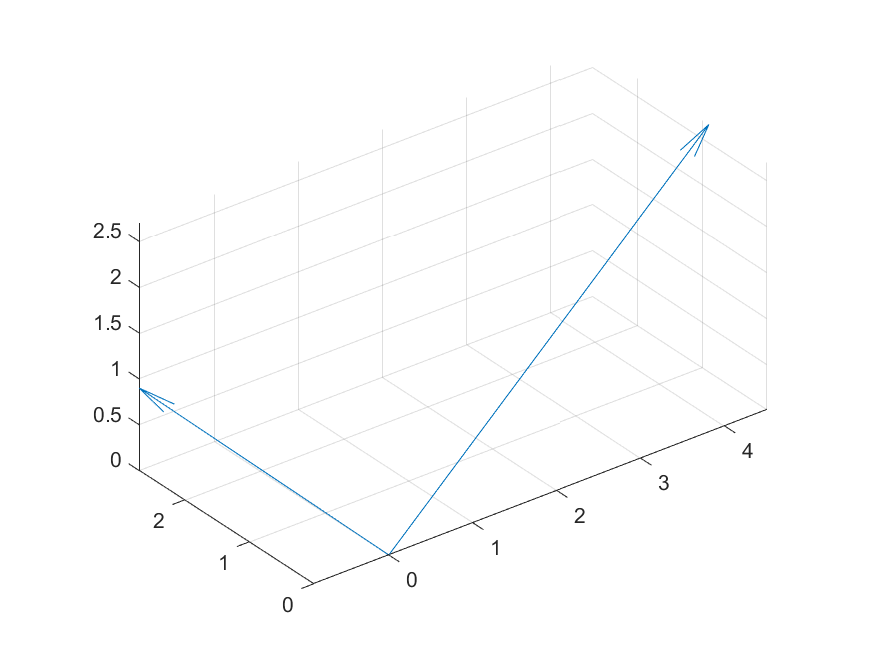
\includegraphics[scale=0.5]{./matlab/chapter-2/sol2.1a.png}
            \end{figure}
            

            \item Find (i) the length of $\bold{x}$, (ii) the angle between $\bold{x}$ and $\bold{y}$, and (iii) the projection of $\bold{y}$ onto $\bold{x}$.
            
\[
    \|\bold{x}\| = \sqrt{\bold{x}^\prime \bold{x}} = \sqrt{5^2 + 1^2 + 3^2} = 5.9161
\]

\[
    \bold{x} \cdot \bold{y} = \left\|\bold{x}\right\| \left\|\bold{y}\right\| \cos{\theta} 
    \Rightarrow \theta = \cos^{-1}{\left(\frac{\bold{x} \cdot \bold{y}}{\left\|\bold{x}\right\| \left\|\bold{y}\right\|}\right)} = \cos^{-1}{\left(\frac{1}{5.9161 \times 3.3166}\right)} = 87.0787 \degree
\]
MATLAB code \texttt{acosd((x'*y)/(norm(x)*norm(y)))} returns the angle in degrees.

\[
    \text{comp}_{\bold{x}}\bold{y} = \frac{\bold{x} \cdot \bold{y}}{\left\| \bold{x} \right\|}
\]

\[
    \text{proj}_{\bold{x}}\bold{y} = \text{comp}_{\bold{y}}\bold{x}\left(\frac{\bold{x}}{\left\|\bold{x}\right\|}\right) = \left(\frac{\bold{x} \cdot \bold{y}}{\left\| \bold{x} \right\|}\right) \left(\frac{\bold{x}}{\left\| \bold{x} \right\|}\right) = \left(\frac{\bold{x} \cdot \bold{y}}{\left\| \bold{x} \right\|^2}\right) \bold{x} = \left(\frac{1}{35}\right) \begin{bmatrix}
        5 \\
        1 \\
        3
    \end{bmatrix} =
    \begin{bmatrix}
        5/35 \\
        1/35 \\
        3/35
    \end{bmatrix}
\]

            \item Since $\bar{x} = 3$ and $\bar{y} = 1$, graph $[5-3, 1-3, 3-3] = [2, -2, 0]$ and $[-1-1, 3-1, 1-1] = [-2,2,0]$.
            
        \begin{lstlisting}
    starts = zeros(2,3);  % Starts at the origin.
    ends = [(x-mean(x))'; (y-mean(y))'];  % Ends at the point. Subtract the mean values.
    
    % quiver3 args are x,y,z,u,v,w. x,y,z are the start positions and u,v,w are
    % the end positions.
    b = quiver3(starts(:,1), starts(:,2), starts(:,3), ends(:,1), ends(:,2), ends(:,3));
    axis equal
    saveas(b, '.\applied-multivariate-statistics\solutions\chapter-2\sol2.1c.png', 'png')
        \end{lstlisting}

        \begin{figure}[H]
            \centering
            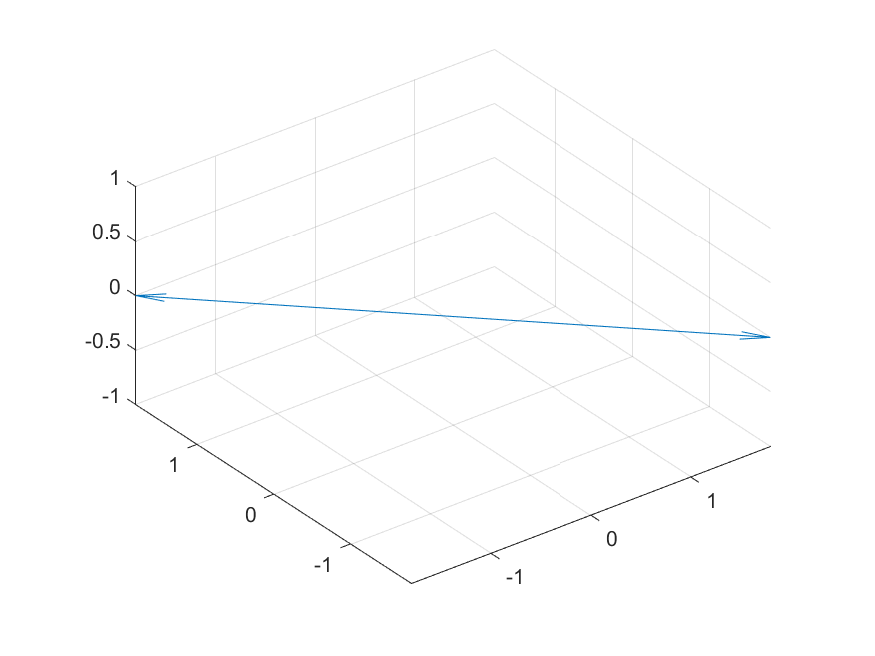
\includegraphics[scale=0.5]{./matlab/chapter-2/sol2.1c.png}
        \end{figure}

        After subtracting off the respective means from both $\bold{x}$ and $\bold{y}$ (centering), the results of both vectors exist on the same line through the origin, but point in different directions.
            
        \end{enumerate} 